\section{Resultat}

\import{Tabeller}{all}

% \subsection{Inklinasjon}

\import{Tabeller}{inklinasjon}

\begin{figure}[h!]
    \centering
\begin{subfigure}{.5\textwidth}
    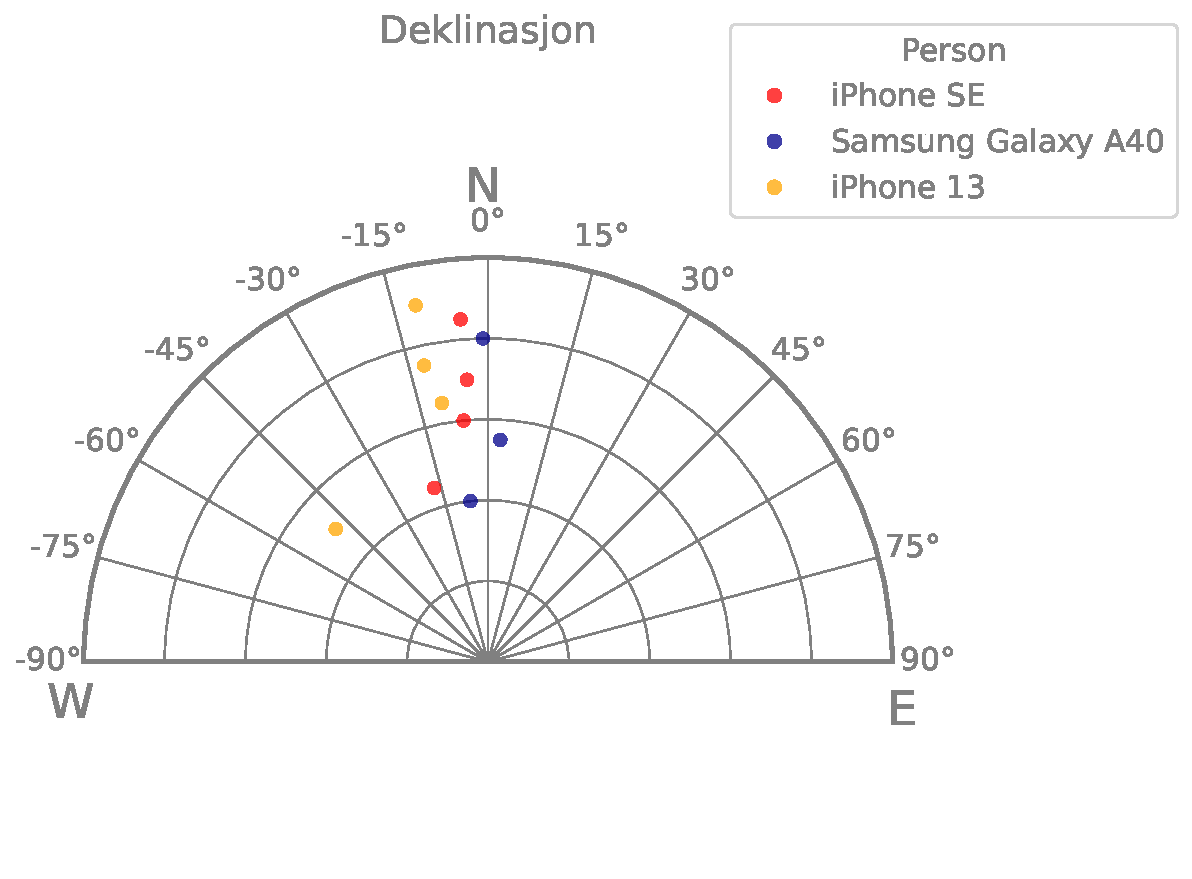
\includegraphics[width=1\textwidth]{Plots/declination.pdf}
    \caption{Plott av deklinasjon for de ulike målesettene. \\
    Fargen angir hvilken telefon som ble benyttet.}
    \label{fig:plot_declination}
\end{subfigure}%
\begin{subfigure}{.5\textwidth}
    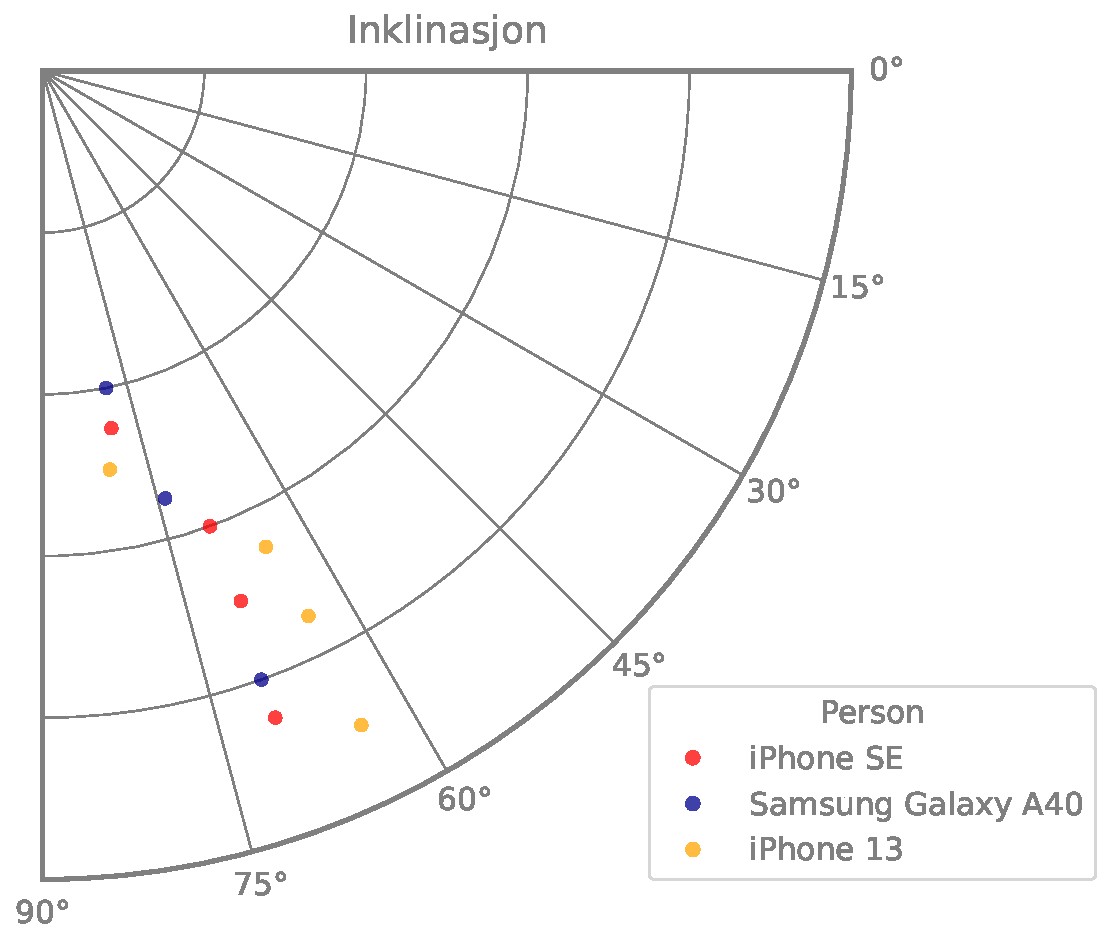
\includegraphics[width=1\textwidth]{Plots/inclination.pdf}
    \caption{Plott av inklinasjon for de forskjellige målesettene. \\
    Fargen angir hvilken telefon som ble benyttet.}
    \label{fig:plot_inklination}
\end{subfigure}
    \caption{Deklinasjon og inklinasjon}
    \label{Ink_og_dek}
\end{figure}


% \subsection{Deklinasjon}

\import{Tabeller}{deklinasjon}

\begin{figure}[h!]
    \centering
    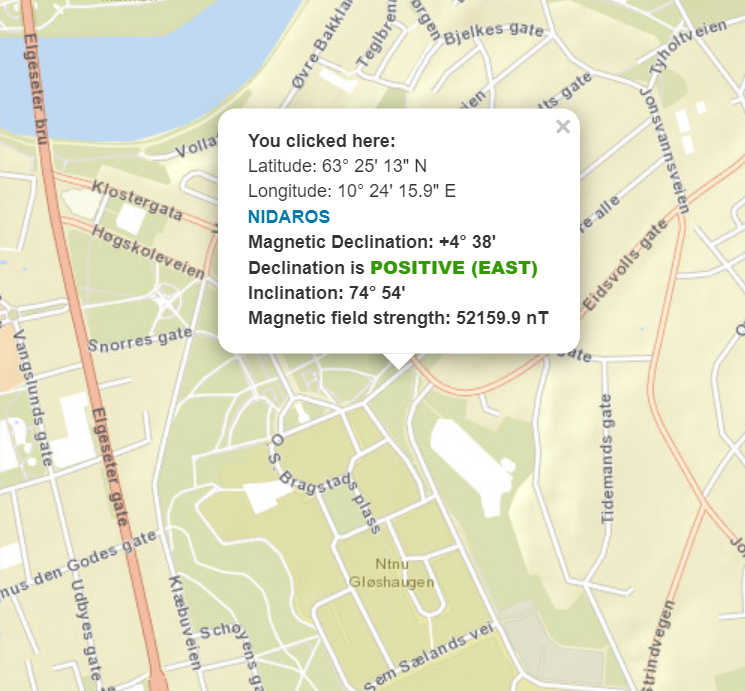
\includegraphics[width=0.5\textwidth]{img/WMM.png}
    \caption{Magnetisk deklinasjon og inklinasjon på vestre side av av broen som krysser Eidsvolls gate langs Øvre alle ifølge \href{https://www.magnetic-declination.com/}{magnetic-declination.com}. Denne nettsiden bruker World Magnetic Model 2020. \cite{magnetic_declination}}
    \label{fig:WMM}
\end{figure}
